\placelogofalse
\begin{frame}{Lattice Boltzmann method (LBM)}
\begin{columns}
\column{0.48\linewidth}
\begin{outline}
\1 $D$ dimensional grid of points $x$
\1 Microscopic velocity distribution $f(x, t)$ at each point
\1 $Q$ discrete microscopic velocities $c_i$
\1 Macroscropic properties are moments of microscopic distributions
\1 Advance time with two operators, 
\textit{streaming} and \textit{collision}
\end{outline}

\column{0.48\linewidth}
\centering
\begin{center}
  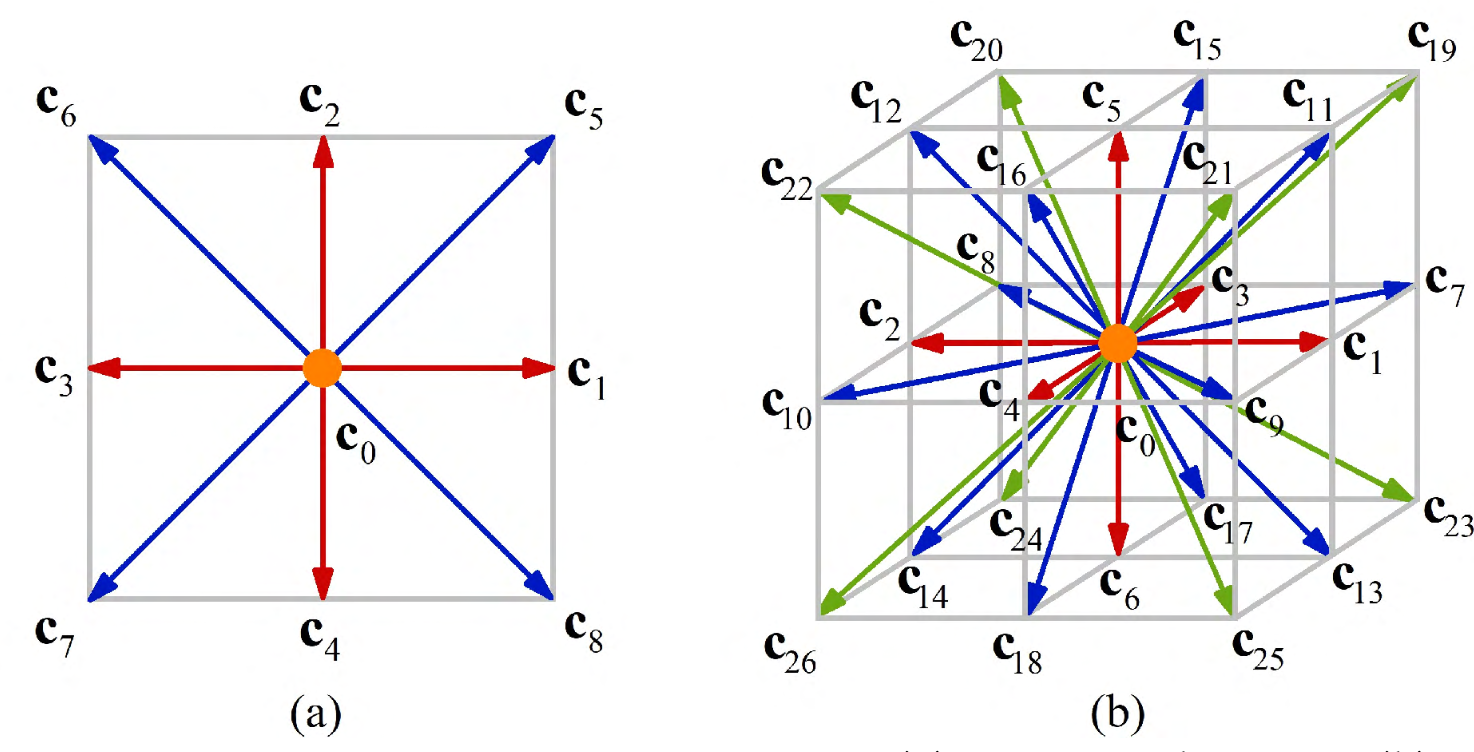
\includegraphics[width=0.9\linewidth]{lattice_figure.png}

  \begin{align*}
  \rho(x, t) &= \sum_{i = 0}^{Q - 1} f_i(x, t) \\
  \rho(x,t)u(x,t) &= \sum_{i = 0}^{Q - 1}c_i f_i(x, t)
  \end{align*}
\end{center}
\end{columns}
\blfootnote{Figure from \cite{Li2020}}
\end{frame}
\placelogotrue

\begin{frame}{Storage and Streaming}
\begin{columns}
\column{0.48\linewidth}
\begin{outline}
\1 Non-local operator
\1 Send velocity distribution to neighbor point
\1 Information travels at speed of sound!
\1 How are distributions stored? (AoS, SoA)
\1 Double buffered?
\end{outline}

\column{0.48\linewidth}
\centering
  \begin{center}
    \includegraphics[width=0.4\linewidth]{stream_0.png}
    \includegraphics[width=0.4\linewidth]{stream_1.png}

    \includegraphics[width=0.6\linewidth]{stream_2.png}
  \end{center}
\end{columns}
\end{frame}


